Betrachten Sie folgendes (valide) Klassendiagramm:



\begin{centering}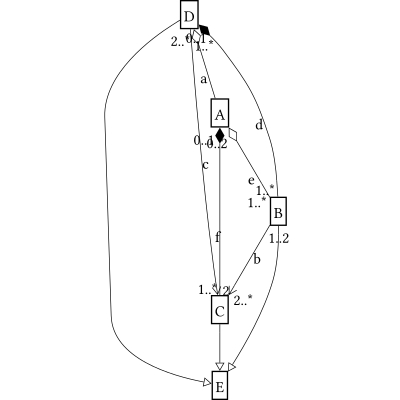
\includegraphics[min width=0.4\textwidth=0.6\textwidth,min height=0.4\textwidth=0.6\textwidth,keepaspectratio,max width=0.9\textwidth,max height=0.9\textwidth]{56/cdda6a11549572837c138bba9a1c158456881717bc6d103466234eed613892341d11af83b04c596701db35357ce8aed00a3a92e08161.pdf}\end{centering}



und das folgende (dazu passende) Objektdiagramm:



\begin{centering}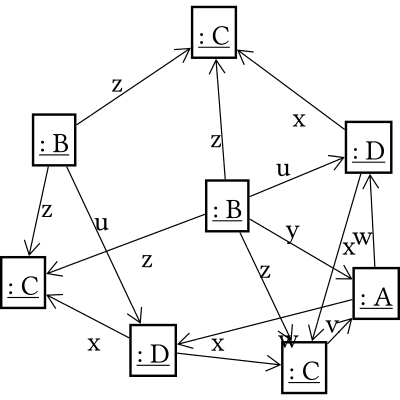
\includegraphics[min width=0.4\textwidth=0.6\textwidth,min height=0.4\textwidth=0.6\textwidth,keepaspectratio,max width=0.9\textwidth,max height=0.9\textwidth]{56/od3175862b30d91dbf6f4cd4e63838eb8da4661f8ad659a52a837e1e36d155f90210.pdf}\end{centering}



Welche Beziehung im Klassendiagramm (CD) entspricht welchen Links im Objektdiagramm (OD)? 
 Geben Sie Ihre Antwort als eine Zuordnung von Beziehungen im CD zu Links im OD an. 
 Um anzugeben, dass a im CD zu x im OD und b im CD zu y im OD korrespondieren, schreiben Sie die Zuordnung als:\begin{verbatim}[(a,x),(b,y)]\end{verbatim}

Bitte beachten Sie: Links sind bereits vollständig und korrekt gruppiert, d.h., alle Links mit dem selben Namen (and auch nur Links mit dem selben Namen!) im OD entsprechen genau dem selben Beziehungsnamen im CD.

Deshalb sollte kein Link- oder Beziehungsname mehr als einmal in Ihrer Zuordnung auftreten.

Bitte beachten Sie: Klassen werden hier vereinfacht dargestellt. 
 Das heißt, sie bestehen aus einer einfachen Box, die nur den Klassennamen enthält, aber keine Abschnitte für Attribute oder Methoden. 
 Trotzdem sollten Sie diese vereinfachten Klassendarstellungen als valide Klassen ansehen.

Da Navigationsrichtungen verwendet werden, beachten Sie bitte, dass Aggregationen und Kompositionen nur vom \glqq{}Teil\grqq{} zum \glqq{}Ganzen\grqq{} navigierbar sind, d.h., sie sind nicht in der entgegengesetzten Richtung navigierbar!

Bitte beachten Sie: Beim Bewegen über oder Klicken auf Kanten / Knoten bzw. ihre Beschriftungen werden die jeweils zusammengehörenden Komponenten hervorgehoben.

